\section{Indoor Air Quality and Vapor Intrusion}
% History and perspective on indoor air quality
Concerns about air quality are as old as civilization itself, ranging from beliefs that disease is caused by bad air - a \textit{miasma}, to more recent concerns about exposure to combustion particulates, radon gas, or other air-borne pollutants.
Since industrialization the number of potential hazardous pollutants has increased significantly, followed by increased concerns about air quality.
At the same time, people now spend more time indoors now than ever before, with Americans spending up to 90\% of their waking time indoors\cite{klepeis_national_2001}.
This change in human habitation has put a special emphasis on indoor air quality.\par

Some early scientific inquiries into indoor air quality focused on pollutant sources that were generated in the home, e.g. by heating and cooking systems, and these types of pollutants are still relevant today, but of particular concern in developing countries\cite{craig_d._hollowell_combustion-generated_1976,world_health_organisation_who_2014}.
Many buildings materials can also cause indoor air quality issues, with exposure to asbestos fibers being perhaps one of the more famous examples of this.
Mold is another common indoor quality concern\cite{world_health_organisation_who_2009}.\par

% Introducing Rn
In the 1970s, to address the growing public health concerns, research began into the potential exposure to radioactive radon gas in buildings.
Radon gas, which is generated by the decay of naturally occurring uranium in soils and rocks, was found to be able to enter overlying building and expose the inhabitants.
This phenomena came to the public attention in the mid 1980s, after a Pennsylvanian nuclear power plant worker set off radioactivity sensors at the plant, the actual cause of which was the high concentration of radon gas in the workers home\cite{noauthor_health_nodate}.
Exposure to radon gas can significantly increase the risk of developing lung cancer, and is to this day the second leading cause of lung cancer in many countries\cite{gaskin_janet_global_nodate}.
With the discovery of radon intrusion into buildings, it did not take long for the same concerns to be extended to the entry of anthropogenic contaminant vapors - vapor intrusion (VI).\par

Vapor intrusion is the migration of contaminant vapors from a contaminant source, often contaminated groundwater, into the overlying buildings.
These vapors evaporate from the contaminated groundwater and enter through cracks in the building foundation, gaps between walls and floors, sump pits, or other openings\cite{u.s._environmental_protection_agency_oswer_2015}.
In these aspects, VI is more or less similar to radon intrusion, and thus much of the early VI research was heavily influenced by the work done by radon intrusion researchers.
This is largely true to this day, but vapor intrusion differs in some non-trivial ways, that make it an unique issue.
Many of these differences stem from the properties of the contaminants themselves, and from the fact that many of the VI contaminants that we concern ourselves with, mainly volatile organic compounds (VOCs) and chlorinated solvents, are of anthropogenic origins.\par

One difference is that radon is unstable, and has a half-life of around 3.8 days (at least Rn\textsuperscript{222}, the only naturally occurring isotope of radon), and it follows that radon accumulation will be naturally mitigated, which is not the case with other contaminants\cite{schumacher_fluctuation_2012}.
The closest analogy is that certain VOCs of VI concern are able to be biodegraded by bacteria in the soil, but this effect can vary significantly as this process is oxygen limited\cite{u.s._environmental_protection_agency_oswer_2015,abreu_simulating_2006}.\par

A more significant difference is the anthropogenic origin of VI contaminants.
In VI, we often are concerned with a contaminated groundwater source underneath the afflicted building, and the source of the groundwater contamination typically originates from some contaminant spill at one or more sites in the surrounding area.
Thus, a large number of buildings may be impacted by VI via a single contaminant source.
The origins of such spills are numerous, but any activities that employ the contaminants of VI concern are possible culprits\cite{u.s._environmental_protection_agency_oswer_2015}.
In the United States (US), the Environmental Protection Agency (EPA) maintains a list of significantly polluted sites throughout the country, so called Superfund sites, and as of 2020 there are 1335 recorded sites, many of which contain the contaminants of concern\cite{us_epa_current_2015,u.s._environmental_protection_agency_oswer_2015}.
Additionally, many of the contaminants of concern do not readily degrade, and legacy contamination is an issue\cite{u.s._environmental_protection_agency_oswer_2015}.
It should also be noted that VI from a contaminated groundwater is only one type of contaminant source, with leaky subsurface tanks, spills into soils, etc., likewise being contaminant sources of concern.
Figure \ref{fig:vapor_intrusion} shows some of the VI processes.\par

\begin{figure}[htb!]
  \centering
  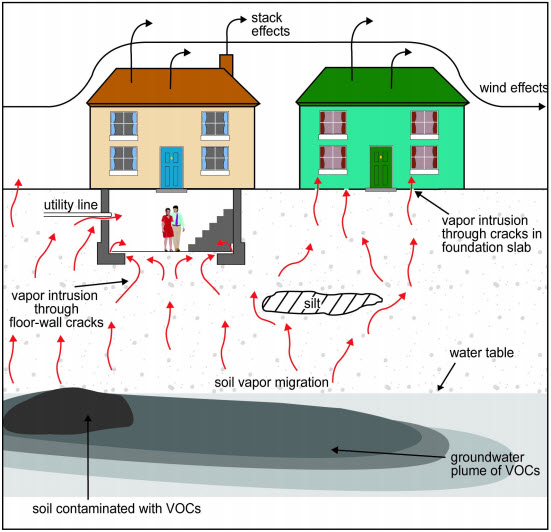
\includegraphics[width=0.75\textwidth]{vaporintrusion.jpg}
  \caption[Overview of vapor intrusion]{Vapor intrusion into a building can occur through a variety of means, from a variety of sources. Figure from the EPA\cite{us_epa_what_2015}.}
  \label{fig:vapor_intrusion}
\end{figure}

In VI, some common contaminants of concern are chlorinated solvents such as trichloroethylene (TCE), tetrachloroethylene (PCE), or chloroform.
Various other organic compounds such as benzene, or other petroleum products are also of concern.
Out of the various VI contaminants, TCE has emerged as of perhaps particular concern.
TCE is an excellent degreaser and has seen extensive use as such, and has been commonly used by dry cleaners, the military, auto repair shops etc\cite{u.s._environmental_protection_agency_oswer_2015}.
The concern over TCE is partly due to its associated cancer risk and partly because it was recently hypothesized to possibly play a role in birth defects.
A review study by \citeauthor{makris_systematic_2016}\cite{makris_systematic_2016} showed that TCE may be associated with increased risk of congenital heart defects (CHD), but a more recent study by \citeauthor{urban_systematic_2020}\cite{urban_systematic_2020} concluded that, mainly due to reproducibility issues and new studies, there is not adequate evidence to support that TCE causes CHD.
Regardless, it is carcinogenic and surprisingly despite the concerns about its health effects, its use remains legal.\par

Considering the widespread existence of potential VI sites and the associated health concerns, an industry for identifying and characterizing these sites and either remediating or mitigating them has emerged.
This is particularly true in the US, where the law dictates that the responsible party of the contaminant spill or release is liable for cleanup and mitigating human exposure.
In this situation significant effort is spent on determining liability.
Determining if VI occurs at a particular site, as we will see in this work, is not easy, and while VI has been studied for decades, many questions and challenges remain, in particular with regards to the great spatial and temporal variability that exist both within and between VI sites\cite{u.s._environmental_protection_agency_oswer_2015}.\par
